%*****************************************
\chapter{Vitamin D}\label{ch:vitD}
%*****************************************

%*****************************************
\section{Introduction}
%*****************************************

\subsection{What is vitamin D?}

The human body requires what is called essential nutrients, which are compounds that the body cannot synthesize by itself, or is unable to synthesize in large enough quantities. These essential nutrients consist of macro-nutrients, vitamins, minerals, choline, and water.

Vitamins are organic molecules that the body needs in small quantities for correct metabolism. They are presented in two groups, water-soluble vitamins, and fat-soluble vitamins. Water soluble means they dissolve in water, while fat soluble means that they dissolve in fat. Vitamin D, along with vitamins A, E, and K, belongs to the fat-soluble group, meaning that they are absorbed through the intestinal tract with the help of fats (also known as lipids). Luckily, vitamin D is already present in fat-rich food such as salmon. Humans need a constant intake of water-soluble vitamins as the body is unable to store them, with the exception of B9 (folate) and B12 (cobalamin). These two vitamins are not technically stored, but they can bind to other proteins and iron, which extends their half-life in blood for about 3 weeks and 3 years respectively.

There are two methods by which your body obtains Vitamin D, sun exposure (pre-vitamin D3) and food intake or dietary supplements (vitamin D2 and D3). Regardless of intake method, vitamin D needs to undergo two chemical transformations known as hydroxylation in order to be activated and do its functions. The first one occurs in the liver and transforms vitamin D into \gls{25ohd}, using 25-hydroxylase. This first form of vitamin D is the variable that we measure in the blood serum later on. The second hydroxylation happens in the kidneys and forms \gls{125ohd}, using 1-$\alpha$-hydroxylase, which is the final and physiologically active form of vitamin D. This form is known as calcitriol. If calcitriol becomes excessive, then is converted to 24,25-dihydroxycholecalciferiol, which is less active. This prevents hypervitaminosis D, and it is why this condition is very rare unless a person takes an insane amount of vitamin D supplements.

Lastly, calcitriol needs to enter the cells; this is where the \gls{vdr} comes into play. This protein is mainly found in the cells of the small intestine, immune system, kidneys, and bones. Calcitriol then binds to VDR, which forms a protein complex that enters the nucleus of cells and binds to DNA, up or down-regulates the expression of hundreds of genes \cite{Nagpal2005, Dusso2005}. This includes calcium absorption (promotes calbindin), bone formation, cell growth \cite{Samuel2008}, and immune function. VDR regulates the production of cytokines (INFLAMMATION SECTION HERE) in the immune system, generally acting as an anti-inflammatory agent, facilitating humoral response (INFLAMMATION SECTION HERE), and leading to homeostasis. In figure \ref{fig:vitVDRimmune} we see an overview of these functions.

\begin{figure}[h!]
{
    \centering
    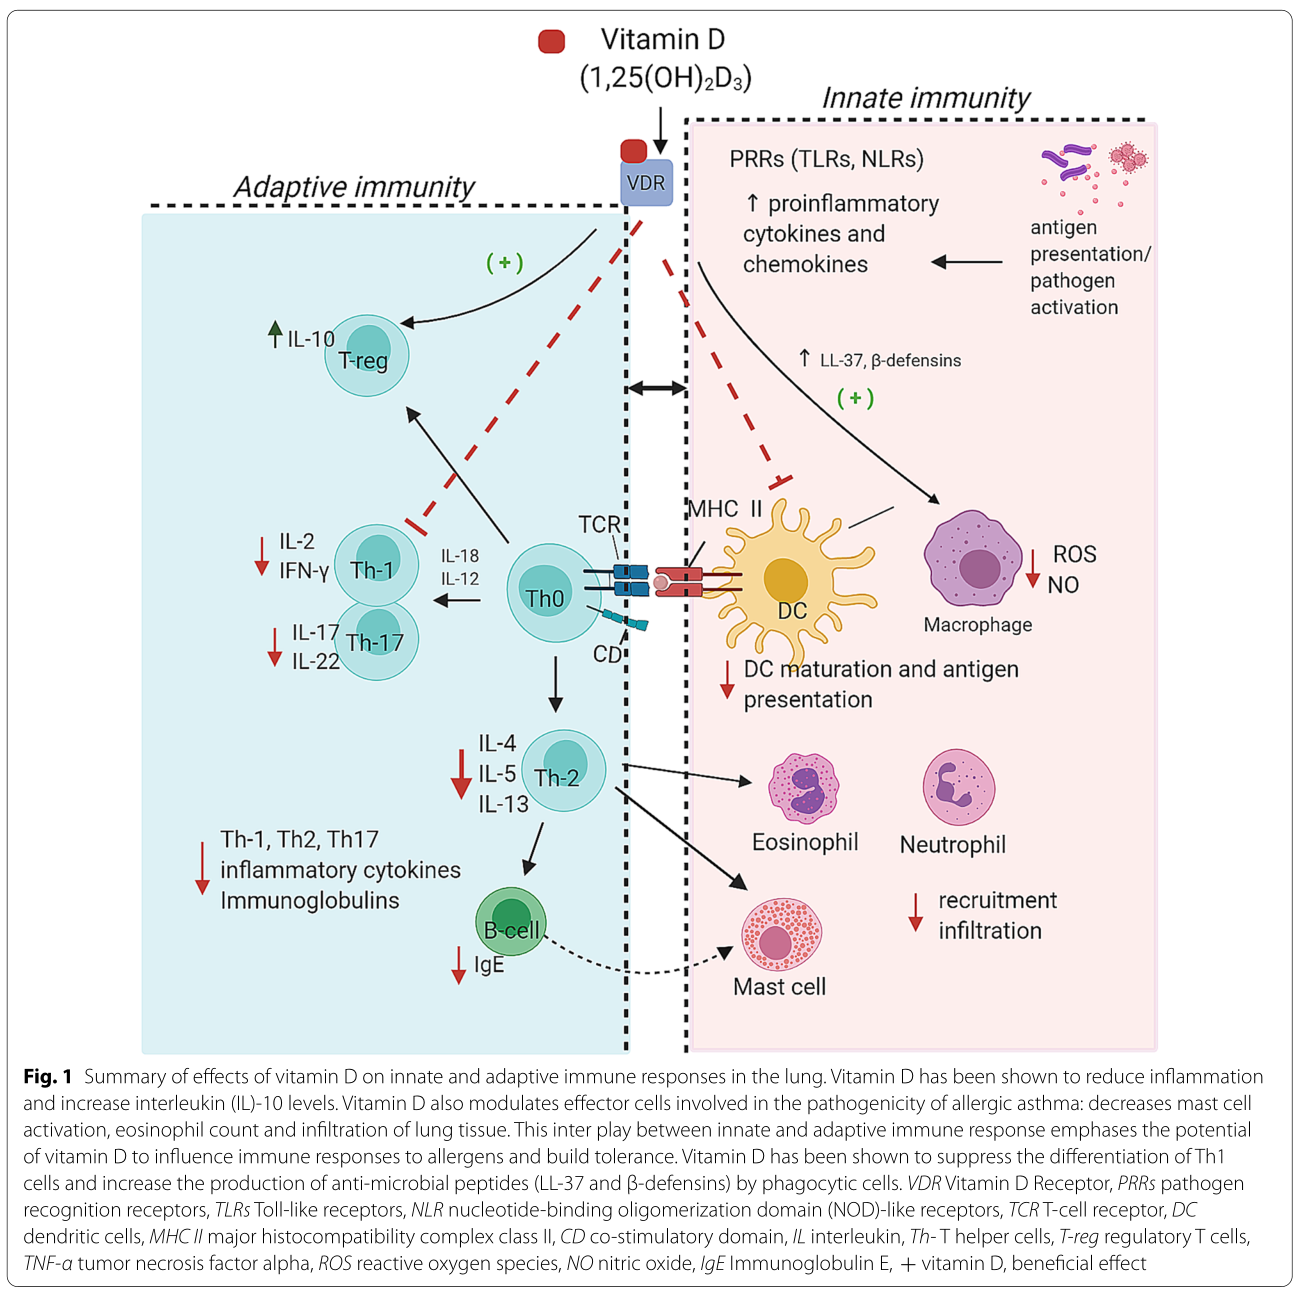
\includegraphics[width=1\textwidth]{figures/Vitamin D/VDRImmunity.png}
    \caption{Overview of vitamin D effects on the immune system. Figure reproduced from "Recent advances in vitamin D implications in chronic respiratory diseases" \cite{Gaudet2022}} 
    \label{fig:vitVDRimmune}
}
\medskip
\end{figure}

Both vitamins D2 (ergocalciferol) and D3 (cholecalciferol) raise 25(OH)D levels. The metabolism and actions of vitamins D2 and D3 are identical, and they only differ in the chemical morphology present in their side-chain structure. Evidence suggest that vitamin D3 increases 25(OH)D levels greater and longer than vitamin D2 \cite{ref:Tripkovic2012, ref:Lehmann2013, ref:Logan2012, ref:Tripkovic2017}. Dietary supplements of 25(OH)D3 are three to five times as potent as vitamin D3 supplements \cite{ref:GraeffArmas2019, ref:QuesadaGomez2018}; but as far as I know, there are no available commercial supplements of this type. In any case, all form of dietary vitamin D is absorbed in the small intestine via passive diffusion using intestinal membrane carrier proteins \cite{ref:Silva2017}. As stated before, the presence of fat helps the diffusion and absorption of vitamin D, although some vitamin D can still be absorbed without fat.

There are two primary functions for vitamin D, to absorb calcium and phosphate from the gut into the blood; and to inhibit \gls{pth} production.

\subsection{Calcium}
\label{vd:calcium}

Calcium ions (Ca2+) are an indispensable neurotransmitter and play a critical role in muscle contraction. Without proper calcium levels in your blood, your heart will just stop working or work incorrectly. On top of that, calcium promotes healthy bone mineralization and bone growth. Finally, calcium promotes sperm hyper-activation, causing them to increase their mobility by "shaking" more violently, increasing their chances of reaching the oocyte, thus a better chance of fertilization \cite{ref:1_Institute_of_Medicine2011-zg, ref:2_Limongi2017-al, ref:3_680f7627099e40be878db46152ebe484}. Calcium is the most abundant mineral in blood, and the 5th most abundant element in the body after Hydrogen and Oxygen (water), Carbon (every cell wall), and Nitrogen (the backbone of amino acids, RNA, and DNA).

When calcitriol is present in the blood, it stimulates the epithelial cells in the intestine to increase the production of calbindin-D proteins. This increases the absorption of calcium from the brush border to the basolateral membrane, where calcium finally enters the bloodstream. While vitamin D is in charge of absorbing calcium, is not in charge of maintaining healthy levels of calcium in the blood serum. This is the task of PHT. If calcium levels are too low, then PTH:

\begin{itemize}

    \item Binds to osteoblast, which increases \gls{rankl}, which transforms pre-osteoclasts into osteoclasts. Osteoclast literally breaks down your bones apart in order to maintain calcium ions as they should be. The self-destruction of bones might sound brutal but your body prioritizes having a working heart before having a working skeleton. Details of this process are explained in section \ref{in:RANKL}.
    
    \item Make you urinate less calcium by increasing renal re-absorption in the kidneys. More precisely in the distal convoluted tubule. Ultimately, this calcium is reabsorbed into the blood, but in exchange, you will urinate more phosphate.
    
    \item Because you are running low on calcium, it will increase the production of 1,25(OH)2D in the kidney, by increasing the production of 1-$\alpha$-hydroxylase.
    
    \item Because breaking down bones and having too much calcium in the blood is also not good, PTH also inhibits the production of PTH, making a negative feedback loop that prevents flooding your blood serum with calcium everywhere.
    
\end{itemize}

Having too little calcium in blood serum levels could be caused by:

\begin{itemize}

    \item Not eating enough calcium.
    
    \item Your parathyroid gland is not working (hypoparathyroidism), so no PTH to take calcium from the bones into the blood.
    
    \item You are taking too little vitamin D. Even if you drink an entire cow's worth of milk, without activation of the calbindin proteins, calcium can't be absorbed by the gut at significant levels.
    
    \item Your kidneys are not working. If your kidneys don't make calcitriol, you won't have the ultimate form of vitamin D regardless of how much you take from the Sun or food.
    
    \item Your liver is not working. As to a similar reason to the previous point, if the first hydroxylation didn't happen, so can't the second one.
    
    \item Everything is fine, but your calcium is binding to something else. Due to hyperphosphatemia (eating too much bad phosphate, generally in fast food and soft drinks), alkalosis (blood is too acidic, higher albumin, which binds to calcium), or too much fatty acids in the blood.
    
\end{itemize}

On the opposite side, if you have too much vitamin D and too much calcium, then is time to save the calcium, and prevent vitamin D toxicity. This is what Calcitonin is for, which is secreted in the thyroid glands. Calcitonin simply decreases calcium levels by inhibiting osteoclasts, so they don't break down your skeleton anymore. Having too much calcium in the blood is not that dangerous compare to having too little, thus calcitonin has less homeostasis power than PTH and calcitriol.

Having a bit extra calcium is not that bad, and you really need to have a lot of calcium (>3mmol/L) to start showing symptoms, which include short QT intervals (cardiac arrhythmia, too many Ca2+ ions in your heart make current flow to not work as intended due shorter absolute refractory), muscle weakness (Calcium pump not working properly plus an accumulation of lactic acid), kidney stones (they are trying to get rid of the extra calcium constantly, thus leading to calcium deposit on it way out via urine), or depression. This may be due:

\begin{itemize}

    \item  You are taking too much vitamin D and you are eating too much calcium at the same time. Cut down vitamin D and you can take as much calcium as you want, the extra calcium will just abandon your body with the rest of the waste.
    
    \item  Your parathyroid gland is working too much (Hyperparathyroidism). PTH is stealing calcium from your bones way more than it should.
    
    \item  Bad tumors, as they secrete PTH peptides (PTHrP) to mimic PTH, so they can get more calcium, so can grow better.
    
    \item  Your kidneys are working too much, increasing the calcium reabsorption constantly. Normally due to the use of diuretic substances.
    
\end{itemize}


\subsection{Phosphate}

After calcium, the second most common mineral in blood serum is phosphate, present in the inorganic form of phosphorus. This is crucial for the structure of DNA and RNA. Plays a central role in the transportation of energy in the form of ATP. All cellular membranes are composed of phospholipids. Calcium phosphate salts stiff bones and is a central component for healthy teeth development.

Everything discussed before regarding calcium absorption is also applied to phosphate. On top of that, under normal circumstances, low levels of phosphate in blood may also be caused by:

\begin{itemize}

    \item Not eating enough phosphate-rich food
    
    \item The blood is too acidic (acidosis). This might be due to diabetes-related ketoacidosis, alcohol abuse, or severe respiratory alkalosis.
    
    \item The phosphate is binding to something else, such as magnesium or sodium, which happens during electrolyte disorders. This is especially common in patients with chronic kidney diseases as they take phosphate binders.
    
\end{itemize}

Both calcium and phosphate prevent hypocalcemic tetany, a condition similar to tetanus, in which the involuntary contraction of muscles leads to spasms and cramps.


\begin{figure}[h!]

    \centering
    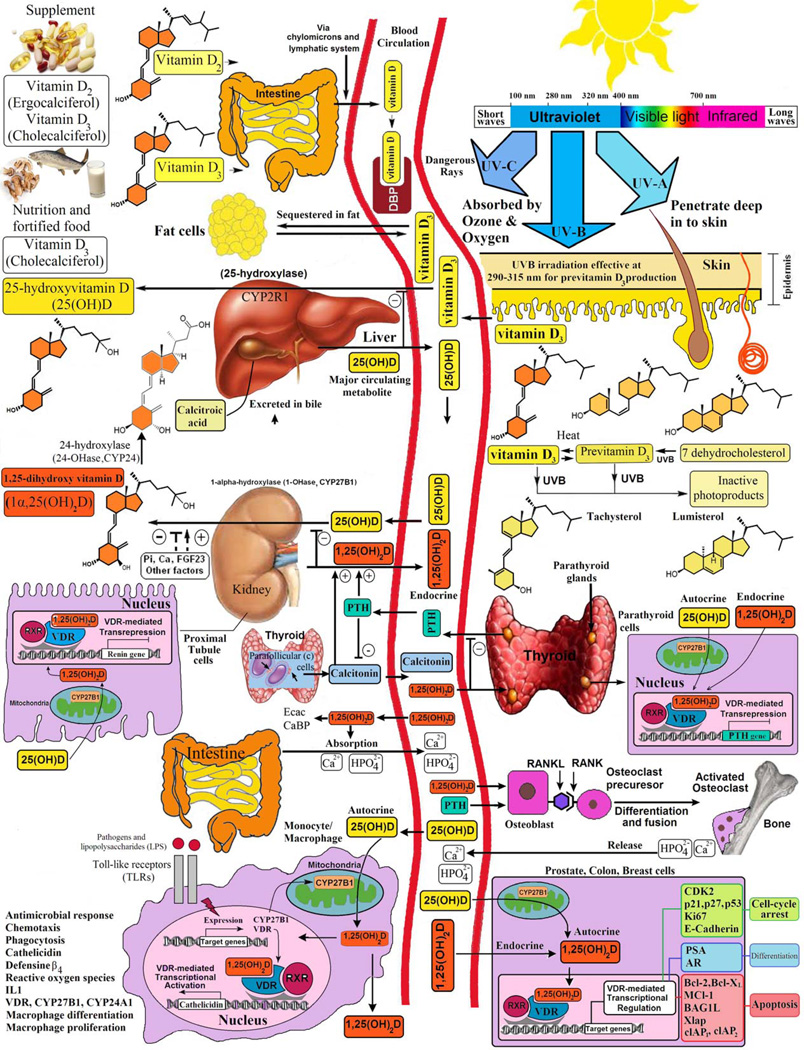
\includegraphics[width=1\textwidth]{figures/Vitamin D/nihms502359f1.jpg}
    \caption{Overview of vitamin D, calcium, and phosphate interactions. Source UNKNOWN!}
    \label{fig:vitDPathways}

\end{figure}

\section{Measuring vitamin D}

\subsection{25(OH)D test}

A 25(OH)D test is virtually harmless, the risk associated with it is the same as with any other blood extraction procedure (bad vein punctuation, the patient fainting because has seen blood, excessive bleeding due to hemophilia or infection in the puncture site) This helps to diagnose a bunch of problems:

\begin{itemize}

    \item If we know that your calcium intake is adequate, check if your calcium absorption is bad due to vitamin D deficiency. If your vitamin D levels are good, it means other conditions affecting calcium absorption are lurking in your body. Similarly, this also helps to measure absorption levels of phosphorus and magnesium.
    
    \item As calcium is taken from the bones, PTH also stimulates vitamin D, which stimulates calcium absorption, thus, paying back to your skeleton the calcium that we just borrowed. Low levels of vitamin D might indicate that your PTH is not working, maybe due to hypoparathyroidism; while high levels of vitamin D might indicate your PTH is working too much, maybe due to hyperparathyroidism.
    
    \item Since it is a fat-soluble vitamin, high levels of vitamin D indirectly indicate low-fat levels. This might happen due to absorption diseases such as cystic fibrosis and Crohn’s disease. It might also indicate a problem in patients where a piece of their digesting system is missing (gastric bypass, shortening of intestines).
    
    \item  To check if the vitamin D supplements that you are taking are actually being processed by the liver and if your levels are back to normal.
    
\end{itemize}



\subsection{1.25(OH)2D test}

As 25(OH)D measures the first hydroxylation, similarly, we could also measure the next hydroxylation and measure the levels of 1,25(OH)2D instead. This is perfectly possible, however, is not common, as the 25(OH)D last much longer in blood and has a higher concentration, it makes the test easier and more reliable than the 1,25(OH)2D counterpart.

\subsection{Standarization}
\label{vitd:vdsp}

Once the blood sample has been extracted from your body, you need to extract the 25(OH)D information from there. Currently, there are two main methods to do so, antibodies and chromatography, and each of these has also several sub-methods that give high variability in the final 25(OH)D levels \cite{ref:Wise2021}. As a result, comparing different studies has become difficult as we will see later in section \ref{lb:epidemiology}. Clinical trials differ way too often from what theoretical data analysis expresses. In essence, any concept, for example, obesity, can express too high, or too low levels of 25(OH)D in different studies, depending on what technique for 25(OH)D analysis is the studying using \cite{ref:Sempos2018, ref:LeFevre2015}

As far as I know, there have been no efforts, or complaints, about 1,25(OH)2D standardization. The leave for a plethora of studies and clinical trials was measuring 1,25(OH)2D instead, which could help to shine some light on the effect of vitamin D.

\subsection{Levels}

As with any other nutrient, vitamin D has upper and lower bound levels which makes for optimal healthy intake, presented in table \ref{tab:vitDLevels}. As stated before, different tests show different levels of 25(OH)D. Furthermore, people depending on their ethnicity, stage of life, bone density, and muscle metabolism, and pregnancy status women, need different levels of intake \cite{ref:Holick2011, ref:Holick2007, ref:Rosen2012, ref:Brown2018}.

\begin{table}[h!]
    \caption{Healthy levels of 25(OH)D in blood serum}
	\centering	
	\begin{tabular}{|l|l|l|} 
		\hline
		\rowcolor[rgb]{1,0.392,0.392} nmol/L & ng/mL    & Significance           \\ 
		\cline{1-2}
		<30          & <12       & Vitamin D deficiency  \\
		30 to 50     & 12 to 20  & Inadequate            \\
		50 to 125    & 20 to 50  & Healthy               \\
		>125         & >50       & Adverse effects       \\     
		\hline
	\end{tabular}
	\label{tab:vitDLevels}
\end{table}

\section{Sources of vitamin D}

\subsection{Sun}

\subsubsection{Electromagnetic waves}

Light is what we call an electromagnetic wave. Electromagnetic waves are classified depending on their wavelength. The energy of a wavelength is given by $E = \hbar \cdot v = \frac{\hbar \cdot c}{\lambda}$. Where $\hbar$ is Planck's constant. V is the speed of the wave which varies depending on the medium in which is traveling (ie: for vacuum, we use "c", the speed of light in vacuum, which is also a constant. Each medium has its own constant). Wavelength is represented by $\lambda$ and is the only variable in the equation. Since wavelength is in the denominator, lower-energy electromagnetic waves have higher wavelengths, while high-energy electromagnetic waves have lower wavelengths. As shown in figure \ref{fig:electroWaves}, the wavelength can vary from kilometers like radio waves to subatomic size like gamma rays.

\begin{figure}[H]
    
    \centering
    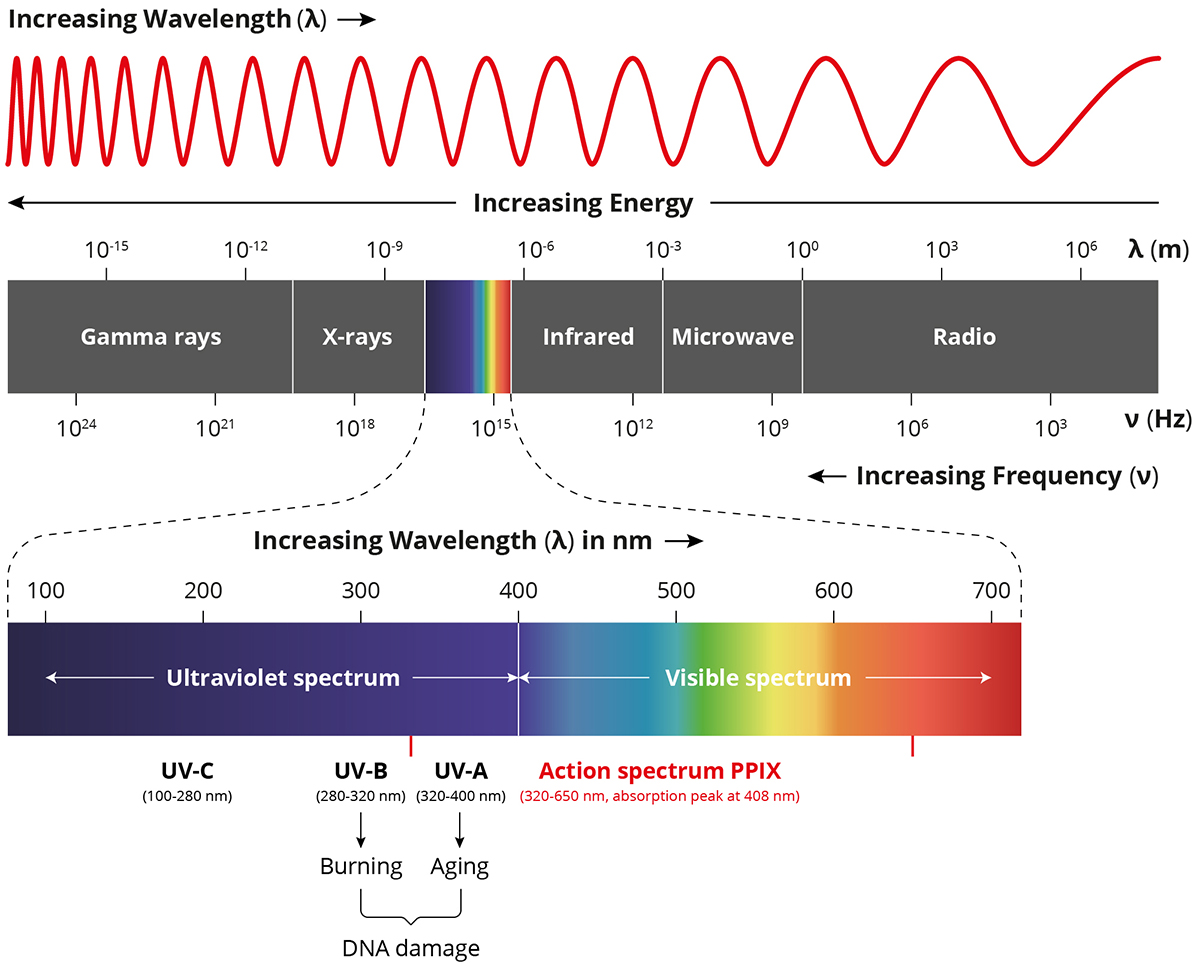
\includegraphics[width=0.8\textwidth]{figures/Vitamin D/Electromagnetic-Spectrum-FINAL.jpg}
    \caption{Overview of the electromagnetic Spectrum. Source UNKNOWN!}
    \label{fig:electroWaves}

\end{figure}

An important differentiation point in energy is what we call "ionizing radiation", this is because, at this point, the electromagnetic waves are able to rip off electrons from the nucleus of the atoms. As a result, DNA and RNA chains will break apart, in most cases leading to cancer in the long run, or even severe radiation poisoning leading to death a few hours after exposure depending on the total dosage received. Ionizing radiation comes in the form of direct ionization (alpha, beta, and antimatter) or indirect ionization (photons such as X-rays or gamma rays, or neutrons). Different atomic elements have different ionizing thresholds, but roughly, ionizing radiation is commonly defined at anything greater than 10eV or lower than 124nm wavelength, as this energy is able to start ionizing oxygen atoms. This wavelength falls in the upper range of UV. The Sun is a very energetic object, but also very dense inside the core. Light in the form of gamma rays that would obliterate all life on Earth is virtually trapped inside the core, and it takes about 500.000 years to transfer that energy from the inner core to the Sun's atmosphere. There, low-energy photons emerge from the Sun, and some of them arrive on Earth. These photons decompose in 50\% infrared or lower radiation, 40\% in the form of visible light, and 10\% in the form of UV radiation or higher.


\begin{figure}[h!]

    \centering
    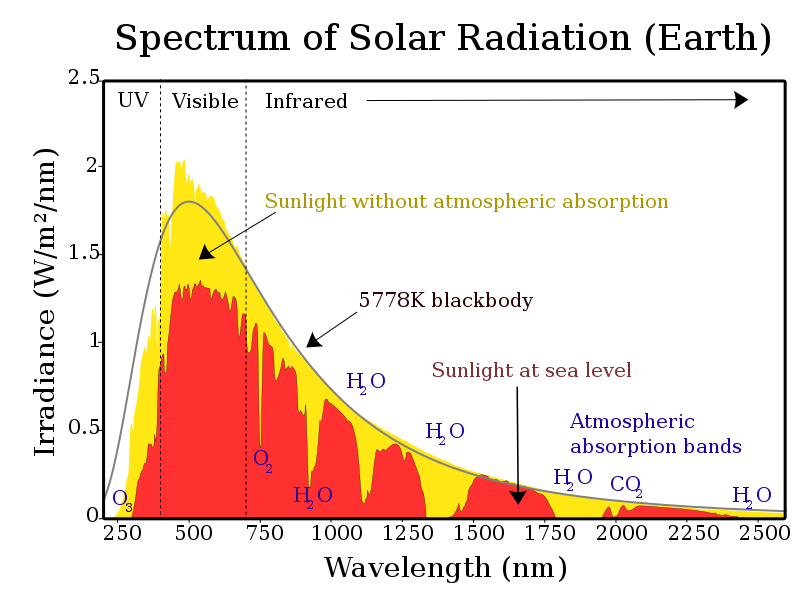
\includegraphics[width=0.8\textwidth]{figures/Vitamin D/800px-Solar_spectrum_en.svg_png.png}
    \caption{Sun's light wavelength decomposition as it reaches the upper atmosphere (yellow) and hit the ground (red). Source: Wikipedia.}
    \label{fig:uvatmosphere}

\end{figure}

Electromagnetic waves are composed of photons, and photons present both the wave and particle properties. We will see later that photons, despise being massless, can strike mass particles, in particular our DNA. There are many effects that different wavelengths can have on matter. In our context, we only care about the excitation of molecular and atomic valence electrons since it is what is involved in vitamin D absorption.

\subsubsection{UV radiation}

\gls{uv}, is a classification of electromagnetic waves based on their wavelength \cite{ref:ISOUV}. Ultraviolet commonly ranges from 100nm to 400nm, although vacuum ultraviolet can be found starting at 10nm. There are many classifications of UV light, some of which are shown in \ref{table:uvExamples}. We only use the \gls{uva}, \gls{uvb}, and \gls{uvc} classification as it  completely encompasses all our health-related interests.

\begin{table}[h!]

	\centering
    \caption{Examples of UV radiation classification according to wavelength.}
	\begin{tabular}{|lll|}
		
		\hline
			\rowcolor[HTML]{CBCEFB} 
				Name & Spectral subcategory & Wavelength range (nm) \\ \hline
				\rowcolor[HTML]{EFEFEF} 
				Ultraviolet          & UV                   & 100 to 400            \\
				Ultraviolet C        & UVC                  & 100 to 280            \\
				Ultraviolet B        & UVB                  & 280 to 315            \\
				Ultraviolet A        & UVA                  & 315 to 400            \\ \hline
				\rowcolor[HTML]{EFEFEF} 
				Vacuum Ultraviolet   & VUV                  & 10 to 200             \\
				Extreme Ultraviolet  & EUV                  & 10 to 121             \\
				Hydrogen Lyman-alpha & HLyman$\alpha$       & 121 to 122            \\
				Far Ultraviolet      & FUV                  & 122 to 200            \\ \hline
	\end{tabular}
    \label{table:uvExamples}
\end{table}

UV radiation is an important differentiation for biological processes because ionizing radiation starts at UV radiation, but not all forms of UV radiation are ionizing. The shorter forms of UVC are ionizing, while UVB and UVA are not. A widely popular belief is that UVA or UVB cause cancer and skin aging due it high energy levels; this is not entirely true. UVA causes damage via indirect DNA damage due to free radicals. UVB causes damage via direct and indirect DNA damage, but neither does it due to ionizing electrons.\vspace{3 mm}

\subsubsection{UVC}

The Earth's atmosphere is really good at blocking UV radiation, roughly blocking 77\% off all UV radiation at maximum intensity when the Sun is at its zenith. UVC is blocked by the ozone layer and oxygen in the atmosphere. In fact, when oxygen is struck with UVC, it forms ozone. Because of this, virtually no UVC ever reaches the Earth's surface. You can still find artificial sources of UVC at ground level, mostly in the form of germicidal UVC lamps which absolutely eradicates all bacterial forms which you shine it upon. UVC radiation cause severe burns to the skin and eye-related injuries in a matter of seconds. Fortunately, UVC exposure injuries usually health within a couple of weeks, and even though UVC is highly energetic, it doesn't have a strong penetration power and the risk of cancer or permanent eye damage is very small. Be aware though that some UVC lamps also emit some amount of UVB radiation, which can cause permanent damage. Overall, UVC is of no concern to us.\vspace{3 mm}

However, germicidal lamps are used in a normal atmospheric environment where oxygen is present. This causes ozone formation, the same as the natural UVC radiation does. Ozone is a toxic gas. Is one of the byproducts of fossil fuel combustion responsible for lung diseases \cite{ref:Stewart2017-sk, ref:badozone2, ref:Jule2018-it} and can lead to skin and eye irritation, and \gls{copd} with chronic exposure \cite{ref:Burnett1997-ra}. As hard to believe as may be, currently many companies offer ozone generators as part of upgrading your air filters; promoting ozone as a good germicidal which it isn't \cite{ref:badozone}. The whole "Ozone is healthy" message is a scam-science pitch-sale at the same level as acupuncture, homeopathy, and all the other common fraudster.

\subsubsection{UVB}

UVB has a higher penetration power and is partially stopped by the ozone layer. UVB is responsible for tanning and vitamin D absorption, which will be discussed later in section \ref{vitDExposure}. Here we are going to focus on the health adverse effects only:\vspace{3 mm}

\begin{itemize}

\item
DNA damage. UVB can break thymine bonds. Normally this is not a problem as they will just bond back to their opposite nucleotide, but if two thymine is adjacent to each other they will be bound to each other instead known as "thymine dimer". This makes a bump in the DNA structure that disrupts normal DNA mechanisms like duplication, translation, or reparation. 

\item
Free radicals. UVB can generate hydroxyl and oxygen radicals. Hydroxyl can damage any macro-molecule (carbohydrates, DNA, RNA, lipids, and amino acids) via oxidative stress. Normal oxygen molecules have 2 electrons, while oxygen radicals only have 1. This cause the molecule to snatch an electron from anywhere else causing a chain reaction of chemical imbalances.

\item
Sunburns. When a cell has undergone DNA damage, it will signal the immune system for self-destruction via apoptosis. The peeling of the skin is the corpse of skin cells that have suffered DNA damage and  has been destroyed. This immune attack creates an inflammatory response responsible for the swelling, itchiness, redness, and pain proper of a sunburn. Sunburns are also known as first-degree burns. Second-degree burns are when blisters start formatting with blood plasma inside due to high temperature. While rare, is possible to get a second-degree burn from the Sun if the temperature is really high or you are in direct contact with a surface being heated by the Sun. But this is not due to UVB radiation, but due to heat transfer caused by infrared light radiation instead.

\item
Melanoma. Due the DNA damage, melanocytes can develop into melanomas. Melanocytes are the skin cells responsible for the production of melanin, people with low melanin are more likely of suffering from melanoma. This is the most dangerous form of skin cancer as it is able to metastasize very quickly due to its proximity to blood and lymphatic vessel.

\item
Vitamin A depletion. Keratinocytes and melanocytes are skin cells that metabolize retinoic acid and transform it into  Vitamin A. Skin can get damaged due to free radicals, when it does, it loses its ability to metabolize Vitamin A (creates new collagen) and generate melatonin (blocking UV damage). Because it is losing its ability to block UV radiation, this makes a positive feedback loop where the skin loses all natural UV protection. 

\end{itemize}

\subsubsection{UVA}

UVA is not blocked at all in the outer layers of the atmosphere and offers no health advantages to us. UVA has the higher penetration power of all the UV spectrums. Another widely known popular belief is that you can get tanned if you take sunbathe behind a common glass (soda-lime glass). This is completely false as almost all forms of glass block UVB radiation to about 90\% or more. However, not all glass stops UVA radiation \cite{ref:Duarte2009}. This effectively means that taking a sunbath at home behind your windows will give you all the negative effects that come with UVA (aging, cancer, etc...) without virtually any of the positive effects of UVB (vitamin D synthesis). Normal glass usually blocks about 25\% of UVA radiation, but other forms of glass exist that block it entirely. Usually, the windshield of cars blocks UVA completely, but this is not true for the side windows glass. Sunglasses and even normal prescribed glasses can have UVA filters.

UVA radiation can also pass through clothes. You need to look for the ultraviolet protection factor for each piece of cloth, but as a general rule, the thicker the material the better, the darker the material the better, cotton and hemp provide low or no protection, nylon and polyester provide excellent protection, any other material provide protection somewhere in between. And of course, UVA protection-specific clothing exists in the market. Sadly, summer is hot, and we use very light clothing at the time of the year when we need protection the most.

Sunscreen usually offers good protection against UVB radiation. You will find the level of protection displayed in the \gls{spf} number of the sunscreen lotion. However, not necessarily offers good protection against UVA radiation. SPF only covers UVB blocking and the lotion can be deceivingly marketed as "Sun protection", when in reality offers no UVA protection at all. As far as I know, there is no standard for UVA protection labeling, and even the SPF standard changes from country to country, so my best advice is to read the label of your sunscreen carefully and investigate the product online. As a general rule, consider the Sun as hostile and trying to kill you all the time, and stay away from it, especially around noon hours.

UVA cause the following problems:

\begin{itemize}

\item Collagen breakdown. The middle layer of the skin (dermis) is mainly composed of collagen and elastin. When collagen breakdown into elastin via matrix metalloproteinases (section \ref{in:MMP1} and \ref{in:MMP10}); this condition is known as elastosis and its symptom is skin aging (wrinkling, sagging, sallowness, hyperpigmentation, dryness, roughness, loss of skin tone).

\item Free radicals. UVA generates hydroxyl and oxygen radicals same as we discussed with UVB. UVA has more penetration power and is more likely to happen due to UVA exposure.

\item Vitamin A depletion. Skin can get damaged via free radicals generated by UVA, the same as it gets damaged with radicals generated by UVB. UVA has higher penetration capabilities which makes it more dangerous. Furthermore, skin can also be damaged by collagen breakdown (UVA exclusive) losing even more capacity to metabolize vitamin A.

\item Cataracts. UVB doesn't have enough penetration power to go through your cornea and lenses, but UVA does. Due to oxidative stress, proteins can clump together at the lenses, reducing transparency. Chaperones can clean these proteins, but is possible to clump protein faster than cleaning them.

\item Cancer. Free radicals can alter DNA structure. We can normally repair DNA damage via a repairing mechanism or scraping a cell entirely including DNA via the immune system. Sometimes this mechanism doesn't work, for example, UVA suppresses T lymphocytes and apoptosis. As a result, malignant tumors proliferate in the form of melanoma, basal cell carcinoma, and squamous cell carcinoma.   

\end{itemize}

\subsubsection{Radiative flux}

In physics, a flux means that something, typically a scalar or vectorial field, is traveling throughout a surface. In our context, we are looking at radiative flux density (also known as power flux density), which is the number of photons that pass through a surface at any given time, measured in $W/m^2$ (W = J/s). Another way of measuring this is through spectral flux density which takes into account the different wavelengths of photons, but in our case, we only care for a very small spectrum (UVB radiation), so we simplify using the radiative flux.

Earth gets closer to the Sun as it orbits it. It will receive more photons thus increasing the flux. However, as Earth's orbit eccentricity is very low (0.017), the difference between the maximum distance to the Sun (1.01 AU), and minimum distance to the Sun (0.98 AU) is small enough to discard completely this effect. The Sun is massively big with respect to Earth, but it is also very far away and appears very tiny in the sky; so tiny that the Sun barely occupies about 0.000068 steradians in the Earth's sky. As such, we can also consider that all photons arriving from the Sun are parallel to each other.

Solar irradiance is the number of photons that arrives from the Sun to Earth. The spherical surface of the upper atmosphere facing the Sun receives about $1300 W/m^2$ on average, while on the ground level is reduced to about $1000W/m^2$. If the Earth were flat and facing the Sun, everywhere on Earth would receive the same energy, and we would have the same season and very similar temperatures everywhere at the same time. This is not true of course. During summertime in the northern hemisphere, we experience more heat from the Sun, while in winter we experience less, even though is the same Sun at a virtually constant distance. This is due to the axial tilt of the Earth with respect to the Sun's light rays. \vspace{1mm}

\begin{figure}[H]

    \centering
    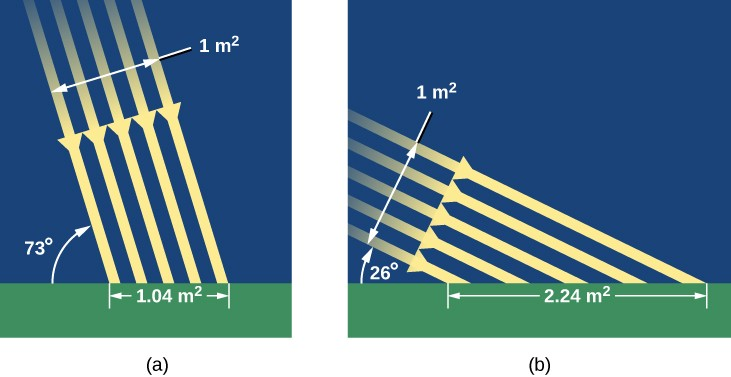
\includegraphics[width=0.5\textwidth]{figures/Vitamin D/OSC_Astro_04_02_Sunray2.jpg}
    \caption{A Sun's beam of light strike the surface with two different angles. Source UNKNOWN!}
    \label{fig:rayTilt}

\end{figure}


In figure \ref{fig:rayTilt}, we see a cross-section of a beam of light coming from the Sun at noon that occupies 1m2. When the beam reaches the ground, if the Sun were at 90º over the ground, the beam would also occupy $1m^2$. Because is slightly tilted, the $1m^2$ beam is spread around $1.04m^2$. So, that 1000W arriving with that beam, now is spread around a bigger area, and the area is receiving slightly less, in particular averaging $964W/m^2$. In winter is much worse, the light is coming very inclined at noon with respect to the summer inclination. As such, those 1000W are spread around a bigger area, in our example, $2.24m^2$. This makes an average of $446W/m^2$. That energy can be reduced further as winter is usually cloudy and the clouds will steal some of that energy too, and the extreme inclination of the beam will make it travel further through the ozone layer and the atmosphere for a bit longer. Which in the case of UV radiation would reduce its power much more than the rest of the spectrum.

In Tromsø, during a sunny day, we receive a comparable amount of photons as in a place around the Earth's equator, but the photons are spread out through a bigger surface. In Tromsø, the Sun elevation during autumn's equinox on the 23rd of September of 2022 is about 20º, one month later is barely 10º, one month later it doesn't rise above the horizon until February when it reaches 10º again, and spring's equinox when it reaches 20º again. Rough calculations here, but from autumn to spring, during the time when we actually have Sun, we receive about $200W/m^2$ on average on clear days. Let's call it $150W/m^2$ for a very clear winter. Of those, barely 10\% is UV. And from those, barely 30\% is UVB, so  roughly $3W/m^2$ worth of vitamin D during the Sun, which translate to about $0.5W/m^2$ on average per day. That is supposing that you go outside fully naked everywhere during winter; realistically, your clothes will cover everything except part of your face and you won't be facing the Sun all the time, so you will barely gain a tiny fraction of that, let's say 0.05W/m2. For comparison, tanning beds bulb's wattage is around 80W for the lowest setting, making 10 min inside a tannin bed the equivalent of 110 days' worth of the half-year winter's Sun in Tromsø. On the bright side (no pun intended), you are going to be very well protected from UV damage here. Further assessment of UV irradiance can be seen in figure \ref{fig:sunirradianceJA}

\begin{figure}[h!]

    \centering
    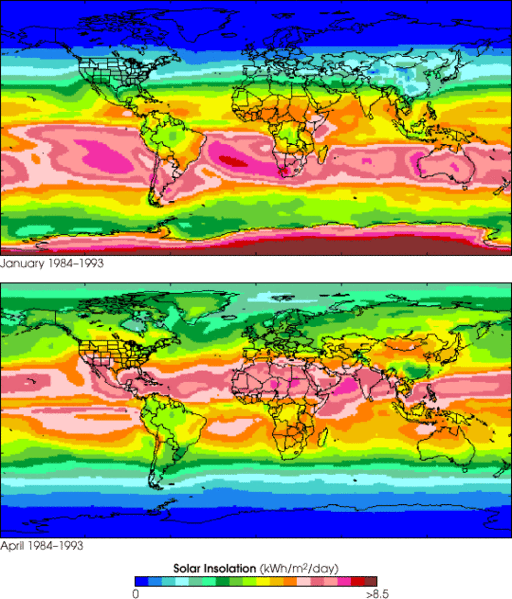
\includegraphics[width=0.5\textwidth]{figures/Vitamin D/512px-Insolation_gif.png}
    \caption{Comparison between solar irradiance between January and April across Earth. Tromsø has 0 in January, while the levels of April are comparably similar to those in the north of Africa during January. Notice that in January, the South Pole has the highest levels possible due to snow reflection. Source UNKNOWN!}
    \label{fig:sunirradianceJA}

\end{figure}
 
\subsubsection{Exposure}
\label{vitDExposure}

Cholesterol is present in various foods: eggs, cheese, shellfish, and organic red meat; which travel through your epithelial cells into your bloodstream. It can be also synthesized or recycled by mostly your liver via the cholesterol biosynthesis pathway and released into your bloodstream. In both cases, it gets oxidized and transformed into pro-vitamin D3 (7-dehydrocholesterol). This is later transported into the epidermis where it is isomerized to pre-vitamin D3 (cholecalciferol) by UVB radiation \cite{ref:Norman1998}.

Pre-vitamin D3 then transforms into vitamin D3 spontaneously. In particular, the B ring of the steroid nucleus structure opens by itself, making a secosteroid that spontaneously undergoes an isomerization transforming pre-vitamin D3 into vitamin D3 (cholecalciferol), which follows the same path as dietary vitamin D3, first bloodstream, then liver, and finally kidneys. \vspace{3 mm}

This is the main process for which the majority of the world population acquires vitamin D3 \cite{1_Institute_of_Medicine2011-zg}. The exposure to sunlight can be increased or decreased via several factors, many of which discussed already:\vspace{3 mm}

\begin{itemize}
    
    \item Being indoor. Any construction material thicker than 2mm blocks UVB quite well, including glass.
    
    \item Having too many clothes. Lighter summer fabric can let through some UVB, but more importantly, dangerous UVA. Work-related clothes can expose you to too much, or too little sunlight depending on the dress code. Also religious impositions particularly on women due to partial or full body covering.
    
    \item Avoiding the Sun, such as walking under a shadow, using umbrellas, or using sunscreen all the time for even short walks.
    
    \item Anything between you and the sky (pollution, clouds, etc...)
    
    \item Sunbathing early in the morning or late in the afternoon, as the sun's rays need to travel further throughout the ozone layer and atmosphere to reach you will lose UVB power along the way.
    
    \item The darker your skin, the lower UVB absorption \cite{ref:1_Institute_of_Medicine2011-zg}.
    
    \item Being old, as skin loses the ability to synthesize vitamin D with age \cite{ref:Chalcraft2020}. Also, old people tend to be less energetic and get out of the house with less frequency.
    
    \item Living in extreme latitudes near the Arctic or Antarctic polar circle due to radiative flux.

\end{itemize}

In contrast, these are the thing that increases UVB absorption:

\begin{itemize}

    \item Snow, ironically, while the Sun during winter has lower radiance flux, snow reflects UV radiation very well and can act as if several tiny Suns are hitting you from several directions at the same time.
     
    \item Tanning beds, emit enough UVB radiation to generate vitamin D.
 
\end{itemize}
   
Each individual in his circumstances is a world of variables that affect UVB exposure. For fair-skinned center Europeans, about 30 minutes of sun exposure, while you walk in shorts and a t-shirt, without sunscreen, at least twice a week, is good enough for vitamin D absorption, and healthy enough to avoid sun damage \cite{ref:Holick2007}. As a general rule, no matter your skin tone, time of the year, or place on Earth; take the time you need to get sunburns wherever you are, divide it by two, and walk around during that time with the least amount of clothes possible that human decency allows in order to get a good and not dangerous UVB bath.\vspace{3 mm}

\subsubsection{UVI}

In order to simplify everything written above the \gls{uvi} was conceived to simplify all possible variables. This is a linear scale that ranks from 1 to 10 (highest risk), indicating the hazard levels of UV radiation at any particular time. You can find this usually along the weather report.\vspace{3 mm}

\subsection{Food}

\begin{table}[h!]

    
    \centering
	\caption{Table with vitamin D levels, per 100 gr, for selected foods belonging to different groups \cite{ref:foodTable}. \gls{rda} based on healthy adult recommendations. }
    \renewcommand{\arraystretch}{1.7}
    \scalebox{0.7}{
	\begin{tabular}{|lrrrr|}
	
		\hline
		\rowcolor[HTML]{CBCEFB} 
		Food name                                                                          & D2+D3 (IU)         & Protein (g) & Energy (kcal) & \%RDA \\ \hline
		\rowcolor[HTML]{BBFFFC} 
		\multicolumn{5}{|c|}{\cellcolor[HTML]{BBFFFC}Fish and sea products}                                                                           \\ \hline
		Caviar, black and red, granular                                                    & 117                & 24.6        & 264           & 20    \\
		Cod liver oil                                                                      & 10000              & 0           & 902           & 1667  \\
		Cod, Pacific, cooked                                                               & 36                 & 17.8        & 82            & 6     \\
		Mackerel                                                                           & 1010               & 18.5        & 305           & 168   \\
		Oyster, Pacific, cooked, moist heat                                                & 2                  & 18.9        & 163           & 0     \\
		Salmon, chinook, smoked                                                            & 685                & 18.3        & 117           & 114   \\
		Salmon, pink, raw                                                                  & 435                & 20.5        & 127           & 73    \\
		Shrimp                                                                             & 2                  & 20.1        & 85            & 0     \\
		Tuna, light, canned in oil, drained solids                                         & 269                & 29.1        & 198           & 45    \\ \hline
		\rowcolor[HTML]{FFCCC9} 
		\multicolumn{5}{|c|}{\cellcolor[HTML]{FFCCC9}Meat and poultry}                                                                                \\ \hline
		Beef, bologna, reduced sodium                                                      & 28                 & 11.7        & 310           & 5     \\
		Canadian bacon, cooked, pan-fried                                                  & 9                  & 28.3        & 146           & 2     \\
		Chicken breast tenders, breaded, uncooked                                          & 9                  & 14.7        & 263           & 2     \\ \hline
		\rowcolor[HTML]{EFEFEF} 
		\multicolumn{5}{|c|}{\cellcolor[HTML]{EFEFEF}Dairy}                                                                                           \\ \hline
		Egg, whole, raw, frozen, pasteurized                                               & 91                 & 12.3        & 146           & 15    \\
		Egg, yolk, raw, frozen, pasteurized                                                & 231                & 15.6        & 291           & 39    \\
		Milk, whole, 3.25\% milkfat, with added vitamin D                                  & 51                 & 3.2         & 61            & 9     \\
		Milk, whole, 3.25\% milkfat, without added vitamin A and vitamin D                 & 2                  & 3.2         & 61            & 0     \\
		Soy milk, unsweetened, plain, refrigerated                                         & 44                 & 2.6         & 43            & 7     \\
		Yogurt, plain, whole milk                                                          & 31                 & 3.8         & 78            & 5     \\ \hline
		\rowcolor[HTML]{9AFF99} 
		\multicolumn{5}{|c|}{\cellcolor[HTML]{9AFF99}Vegetables and fungi}                                                                            \\ \hline
		Brocolli, raw                                                                      & 0                  & 2.8         & 34            & 0     \\
		Carrots, raw                                                                       & 0                  & 0.9         & 41            & 0     \\
		Mushrooms, portabella, exposed to ultraviolet light, raw                           & 1140               & 2.1         & 22            & 190   \\
		Mushrooms, portabella, raw                                                         & 10                 & 2.1         & 22            & 0     \\ \hline
		\rowcolor[HTML]{FFCE93} 
		\multicolumn{5}{|c|}{\cellcolor[HTML]{FFCE93}Fruit}                                                                                           \\ \hline
		Bananas, raw                                                                       & 0                  & 1.1         & 89            & 0     \\
		Orange juice, [...] with added calcium and vitamin D & 40                          & 0.7         & 47            & 7     \\
		Orange juice, raw                                                                  & 0                  & 0.7         & 45            & 0     \\ \hline
		\rowcolor[HTML]{FFFC9E} 
		\multicolumn{5}{|c|}{\cellcolor[HTML]{FFFC9E}Other}                                                                                           \\ \hline
		Almonds, nuts                                                                      & 0                  & 21.2        & 579           & 0     \\
		Bread, oatmeal, toasted                                                            & 0                  & 9.2         & 292           & 0     \\
		Bread, white wheat                                                                 & 0                  & 10.7        & 238           & 0     \\
		Lentils, raw                                                                       & 0                  & 24.6        & 352           & 0     \\ \hline
		
	\end{tabular}
	}
    \label{table:vitDSources}
	
\end{table}


Vitamin D is found in some food. In table \ref{table:vitDSources} we can see a comparison of food high in vitamin D plus other general food groups low in vitamin D. In general, fish has a higher content of vitamin D, namely, salmon, tuna, sardines and mackerel have a higher concentration per kilogram. This amount skyrockets if you take only the liver of the fish. This is not a common part that you find in the supermarket and cook it at home; however fish liver oil can be found everywhere in the form of vitamin D supplements. Meat products are very low in vitamin D in muscle pieces, but once again this varies if you are taking the liver part of the animal; kidneys also have relatively high levels. Butchery shops are more likely to have the livers and kidneys from cattle for sale.

Another source of vitamin D is mushrooms. While not so high naturally, mushrooms exposed to artificial UV light show comparative levels of vitamin D to some fish products and are highest than most. In the market, you might find mushroom powder used as an additive for vitamin D fortification.

Another minor source of vitamin D is milk and dairy product in general. This varies depending on the country's policy on food fortification. Milk however is an excellent choice due to the high concentration of calcium which is ultimately what vitamin D helps your body to absorb. Eggs also offer a source of vitamin D, but only the yolk as it is the only fatty part, and vitamin D is fat soluble.

Breastfeeding doesn't supply the infant with enough vitamin D and additional supplements are required if you exclusively feed your baby with maternal milk. Otherwise, you need to avoid being an overprotecting parent and expose the baby to sunlight \cite{ref:Meena2017-fs}. However, there are organizations such as the \gls{aap} that advise against exposing younger than 6 months babies to sunlight and insist on using vitamin D supplements for babies \cite{ref:Dawodu2012, ref:Davis2007} instead.

Food preparation decrease by about 10\% the amount of vitamin D contained in their raw format counterpart. This doesn't mean that raw food is healthier, you should always cook your fish! Pasteurized and unpasteurized milk have virtually the same vitamin D levels, although pasteurized milk has slightly less of other water-soluble vitamins. Once more, please don't drink unpasteurized milk unless you want a Salmonella party in your digestive tract. Finally, regarding cooking, other vitamins are water soluble and will decrease the vitamin content of the food, such as boiling vegetables. The vitamins don't disappear, they simply remain in the water, so if you are making soup you will still eat them, but if you are steaming vegetables they will evaporate alongside the steam; so calculate your vegetable portions accordingly.

Among European countries, the general rule is that food fortification with vitamin D is allowed and voluntary, although rarely implemented by food brands. Spain and Poland share mandatory fortification for child formula products. In Nordic countries, the policies vary greatly. From Finland having \textit{"mass fortification of milk, margarine/fat spread; fortification of selected brands for yogurt, orange juice, plant-based milk, bread, cereals"} to Norway \textit{"largely prohibited, but voluntary fortification of extra low-fat milk and relatively high intake of cod liver oil and fish oil supplements"}; where Denmark, Iceland, and Sweden policies vary in between \cite{ref:Niedermaier2022-rv}. In the United States, almost all milk and dairy products are voluntarily fortified \cite{ref:Yetley2008-wf}, while in Canada, is mandatory to fortify with 40 IU per 100 g of milk and 530 IU per 100 g of margarine. In both places, baby formula fortification is mandatory with about 80IU per 100 kcal.\cite{ref:1_Institute_of_Medicine2011-zg}

\subsection{Suplements}

Vitamin D supplements are widely available in supermarkets and pharmacies as over-the-counter drugs; these versions already contain more than the daily recommended doses of vitamin D. Higher concentration pills require a medical prescription and are offered to people with bad cases of vitamin D deficiency. There is no difference between taking several low doses of pills or one high doses pill; however as we will discuss in detail later, vitamin D toxicity can be a problem, and you shouldn't self-medicate either.\vspace{3 mm}

If someone is avoiding animal-based products (ie, a vegetarian diet) is very likely that is not taking enough vitamin D via food, and supplements are required. However, some supplements are also animal-based. Vitamin D2 is obtained by irradiating ergosterol in yeast, while vitamin D3 can be obtained by either irradiating pre-vitamin D3 from lanolin which comes from the wool of sheep or using a similar process with lichen instead.\vspace{3 mm}


\section{Deficiency and toxicity}

Vitamin D screening has become more common in primary health care. Previously we stated that sunlight is the method by which most people acquire vitamin D, however, that doesn't mean that people take enough vitamin D either via Sun or dietary sources. In table \ref{tab:vitDeficiencyTable} we can see the prevalence of vitamin D deficiency around the world.\vspace{3 mm}


\begin{table}[h! ]

    \caption{Vitamin D deficiency (25(OH)D < 50nmol/L) prevalence around the world.}	
	\centering

	\begin{tabular}{|ll|}
	\hline
	\rowcolor[HTML]{FFCCCC} 
	Region                  & Prevalence (\%) \\ \hline

	Europe \cite{ref:B_Amrein2020}                 & 40              \\
	\rowcolor[HTML]{EFEFEF} 
	-- Greece \cite{ref:A_Cashman2016}              & 62              \\
	-- Germany \cite{ref:A_Cashman2016}              & 44              \\
	\rowcolor[HTML]{EFEFEF} 
	-- Netherlands \cite{ref:A_Cashman2016}          & 29              \\
	-- Ireland \cite{ref:A_Cashman2016}              & 27              \\
	\rowcolor[HTML]{EFEFEF} 
	-- UK  \cite{ref:A_Cashman2016}                 & 57              \\
	-- Denmark \cite{ref:A_Cashman2016}             & 37              \\
	\rowcolor[HTML]{EFEFEF} 
	-- Finland (foreigners) \cite{ref:A_Cashman2016} & 64              \\
	-- Finland (nationals) \cite{ref:A_Cashman2016}  & 7               \\
	\rowcolor[HTML]{EFEFEF} 
	-- Iceland      \cite{ref:A_Cashman2016}        & 34              \\
	-- Norway  \cite{ref:A_Cashman2016}             & 28              \\
	\rowcolor[HTML]{EFEFEF} 
	---- Tromsø   \cite{ref:A_Cashman2016}          & 19              \\
	
	USA \cite{ref:B_Amrein2020}                    & 24              \\
	\rowcolor[HTML]{EFEFEF} 
	Canada \cite{ref:B_Amrein2020}                  & 37              \\	
	
	Asia \cite{ref:C_Jiang2021}                    & 58              \\
	\rowcolor[HTML]{EFEFEF} 
	Australia    \cite{ref:A_Cashman2016}           & 23              \\
	Africa  \cite{ref:D_Mogire2020}                & 34              \\ \hline
	
	\end{tabular}
	\label{tab:vitDeficiencyTable}
	
	
\end{table}

Different studies use different population backgrounds, testing methods, and times of the year of sampling. This table has been standardized as well as possible for easy comparison following these simplification rules:

\begin{itemize}
    \item Vitamin D deficiency is defined as 25(OH)D < 50nmol/L.
    \item Standardized 25(OH)D levels based on \gls{vdsp} calibration before other tests, if possible.
    \item Summer levels over winter levels (and the other way around in the southern hemisphere)
    \item Adult population (y>18)
\end{itemize}

Ironically, places with high solar irradiance show the highest vitamin D deficiency among their population. One possible explanation for this could be that is common for people to go to work at 08:00 and stay there until 16:00, while driving back and forth to their destination. Because office windows and car windshields block UVB, the person might have the feeling that he has been exposed to Sun all day, but in reality, no UVB has been absorbed. For the rest of the day, the person only has a few hours more of the Sun at its lowest elevation over the horizon. For most cities (where the majority of the population resides), this also means that tall buildings are blocking the Sun, leaving you only a sea of shadows to navigate. Dietary changes over the last years favoring junk food culture didn't help either.

Vitamin D deficiency can be due to any insufficient intake of food or Sun as described so far. But even if you take enough vitamin D, there might be other factors that prevent its absorption. Due to vitamin D being fat soluble, anything that hinders the gut's ability to absorb fat such as liver disease, cystic fibrosis, celiac disease, Crohn’s disease, and ulcerative colitis will lower your vitamin D absorption \cite{ref:Pappa2008}. Some of these diseases can also prevent not only from absorbing vitamin D but even from eating good sources of vitamin D in the first place.

Any medication or drug that interferes with normal liver function, in particular medicines to treat seizures (Phenytoin) causes vitamin D deficiency by interfering with the transformation to 25-hydroxyvitamin D in the liver. \cite{ref:MiratashiYazdi2017, ref:Bell1979, ref:Faridi2010}. \vspace{3 mm}


Obese people don't have a lower capacity to synthesize vitamin D via skin and sun, but the adipose tissue will sequester more of vitamin D. More weight also means more cells that demand more calcium so more need for vitamin D. Furthermore, due to obesity bone stress is higher (more calcium) and muscle strain is also higher (calcium pumps overworking). Overall, evidence suggests that obese people require higher vitamin D \cite{ref:Ekwaru2014, ref:Drincic2013}. Finally, obese people can have bariatric surgery, thus removing part of the digestive tract in charge of absorbing fats and thus decreasing vitamin D absorption \cite{ref:Peterson2016, ref:Chakhtoura2017} .\vspace{3 mm}


Hypervitaminosis D is almost exclusively occurring due to high intake of dietary supplements \cite{ref:Galior2018, ref:Auguste2019, ref:Vogiatzi2014}. Activation of vitamin D3 in the skin gives rise to various non-vitamin D forms that limit the formation of vitamin D3. This is why toxicity due to sun exposure is extremely rare (other conditions can still occurs such as first and second-degree burns, skin aging, cancer, blindness, etc...). Tanning saloons have been linked to causing hypervitaminosis D due to UVB radiation. \cite{ref:Singh2014, ref:Laurent2017, ref:PrezCastrilln2007}
 
The upper limit of vitamin D toxicity can change depending on your maximum intake of calcium. As vitamin D increases the calcium absorption in the gastrointestinal tract, if you take a lot of calcium, this would lead of course to an increase in absorption, developing symptoms of hypercalcemia \cite{ref:Galior2018}. Hypercalcemia due to hypervitaminosis D works the same as regular hypercalcemia and can develop symptoms of nausea, vomiting, muscle weakness, neuropsychiatric disturbances, pain, loss of appetite, dehydration, polyuria, excessive thirst, and kidney stones \cite{1_Institute_of_Medicine2011-zg, ref:Jackson2006, ref:Malihi2019, ref:Malihi2016}. Continuous hypercalcemia can develop for the worse and cause renal failure, and calcification of soft tissue (coronary vessels or heart valves, which by themselves will develop arrhythmias and death).

Other types of harmful vitamin or mineral level events might occur with medication interaction. This includes any medication that reduces fat absorption due to vitamin D being fat soluble, hence not being able to circulate in blood \cite{ref:Gotfredsen2001, ref:James1997-lf, ref:McDuffie2002, ref:Robien2013}. Any medication that modifies cholesterol because pre-vitamin D3 is derived from cholesterol via sun exposure \cite{ref:Robien2013, ref:Schwartz2008, ref:PrezCastrilln2007, ref:Aloia2007}. Any medication that reduces calcium absorption or excretion can modify vitamin D metabolism; this is quite common with both steroids and anti-inflammatories and diuretics (less calcium leaving your body means more calcium inside your body leading to hypercalcemia or hyperparathyroidism) \cite{ref:Robien2013, ref:Crowe1984-or, ref:DRINKA1984, ref:Skversky2011, ref:Lukert1990, ref:deSvaux2002, ref:Buckley1996}. \vspace{3 mm}

With all that said, different endocrine societies, from different countries, have different RDA and different upper limit levels, which also change with time as protocols get updated \cite{ref:Bouillon2017}. In the table \cite{table:vitaminDRDAs} we can see the recommended intake for a healthy individual, sex-independent, pregnancy-independent, and lactation status independent, which tries to summarize all of these different opinions.\vspace{3 mm}

\begin{table}[H]

    \caption{Vitamin D daily recommendation.}	
	\centering
	\begin{tabular}{|l|ll|}
		\hline
		\rowcolor[HTML]{FFAAAA} 
		Age                                 & RDAs           & Upper limits              \\ \hline
		\rowcolor[HTML]{FFFFFF} 
		\cellcolor[HTML]{FFFFC7}0-6 months  & 10 mcg (400 IU) & 25 mcg (1000 IU)  \\
		\rowcolor[HTML]{FFFFFF} 
		\cellcolor[HTML]{FFFFC7}7-12 months & 10 mcg (400 IU) & 38 mcg (1500 IU)  \\
		\rowcolor[HTML]{EFEFEF} 
		\cellcolor[HTML]{EDEDBD}1-3 years   & 15 mcg (600 IU) & 63 mcg (2500 IU)  \\
		\rowcolor[HTML]{EFEFEF} 
		\cellcolor[HTML]{EDEDBD}4-8 years   & 15 mcg (600 IU) & 75 mcg (3000 IU)  \\
		\rowcolor[HTML]{FFFFFF} 
		\cellcolor[HTML]{FFFFC7}9-70 years  & 15 mcg (600 IU) & 100 mcg (4000 IU) \\
		\rowcolor[HTML]{FFFFFF} 
		\cellcolor[HTML]{FFFFC7}70+ years   & 20 mcg (800 IU) & 100 mcg (4000 IU) \\ \hline
	\end{tabular}
    \label{table:vitaminDRDAs}
 
\end{table}



\label{lb:epidemiology}
\section{Epidemiology}


Vitamin D has been related to several diseases, such as bone-related diseases, cancer, cardiovascular diseases, depression, multiple sclerosis, diabetes, and obesity. It's also linked to the modulation of inflammatory processes and testosterone production. However, except for bone-related diseases where there is somewhat strong consensus, there is contradictory evidence between vitamin D levels and the rest of the health issues. This might be due 25(OH)D tests not being properly standardized and poor experiment design \cite{ref:A_Cashman2016, ref:Sempos2018, ref:Sempos20182}.


\subsection{Bone health}

A vitamin D deficiency will lead to a lower amount of calcium and phosphate in the blood. As a result, the main problem with vitamin D deficiency is conditions such as abnormal bone growth, rickets, brittle bone diseases, osteomalacia, or osteoporosis \cite{ref:Elder2014}.

Rickets is a rare disease in developed countries that increase significantly from 10\% to 70\% in places in Africa, the Middle East, and Asia.\cite{ref:ricketstats} And has a higher prevalence in a recent year than in the past, up until the introduction of vitamin D and Calcium supplements in infant food\cite{ref:ricketstats, ref:Uday2017, ref:Munns2016}; a possible explanation for this is the introduction of the immigrant population in first world countries who have different vitamin D absorption rates at an even higher latitude and differences in dietary preferences. Most forms of rickets are due to vitamin D deficiency in children, while severe rickets causes developmental delay, hypocalcemic seizures, tetanic spasms, cardiomyopathy, and dental abnormalities \cite{ref:Uday2017, ref:Munns2016}. Almost all patients with rickets had been partially or exclusively breastfed \cite{ref:Uday2017, ref:Thacher2013}.

Osteomalacia is the same as rickets, but we use rickets for children and osteomalacia for adults. There are different definitions and diagnostic criteria to define osteomalacia, but prevalence is about 3.7\% with a higher rate in women \cite{ref:CAMPBELL1984}.

Bones are constantly being destroyed and built again. However, as people grow older, the ratio in which they are destroyed is higher than being built again. Over time, bone density plummet, and osteoporosis develop. Osteoporosis is characterized by the deterioration of bone tissue leading to bone fractures. About 15\% of people older than 50 and 70\% older than 80 suffer osteoporosis worldwide \cite{ref:osteoporisisstats}. Osteoporosis is caused by the lack of calcium intake, while osteomalacia and rickets are caused by the lack of vitamin D intake; however, a lack of vitamin D intake contributes to the severity of osteoporosis \cite{ref:1_Institute_of_Medicine2011-zg}.

For the general older adult population, some studies show that vitamin D and calcium supplementation increase slightly bone density, display reduces fracture rates. \cite{ref:Chung2009-wl, ref:1_Institute_of_Medicine2011-zg, ref:Yao2019, ref:Bouillon2021}, while other studies show no difference \cite{ref:Kahwati2018, ref:AMADavid2018, ref:Gallagher2018, ref:Bolland2018, ref:AMAGrossman2018, ref:GuirguisBlake2018, ref:LeBoff2022, ref:Bouillon2021} . \vspace{3 mm}

For the United States, bone density, mass, and fracture risk are correlated with 25OHD in white individuals and Mexicans but not for black individuals \cite{ref:Brown2018, ref:Aloia2019, ref:Aloia2005}.


\subsection{Muscle weakness}

Vitamin D assists in the development of muscle fibers. Proper support of the bone structure is needed for optimal bone health, so indirectly, vitamin D also helps bone development not only via calcium absorption but also due to muscle growth. Inadequate levels of vitamin D can lead to myopathy (muscle weakness). Sadly, experiments with vitamin D supplements also include calcium supplements. As such, being able to differentiate between the advantages of calcium and the advantages of vitamin D independently is challenging.

Studies are also not standardized in the amount of nutrients or the time in which they are administered; this is important as nutrient absorption varies with the time of the day and with the food that you are eating. For example, calcium inhibits iron absorption (don't eat meat with cheese), while vitamin C enhances iron absorption \cite{ref:Li2020, ref:Lynch1980, ref:Li2020}(eat meat with orange juice instead). Another example is that proteins need carbohydrates to be absorbed, or as discussed before, vitamins can be water or fat-soluble, and each group requires a different food setup to maximize absorption; all of these variables are rarely taken into account during the intake of supplements in studies.

For the general population, studies have shown either inconsistencies \cite{ref:screeningErin2014} on the effects of vitamin D supplementation with respect the muscle strength and muscle decline, or no correlation \cite{ref:Shea2019,ref:Vaes2018}.


\subsection{Cancer}

Some studies suggest that vitamin D inhibits cancer formation (carcinogenesis) and slows tumor growth. They also suggest that it has an anti-inflammatory effect, can modulate the immune system, triggers cells to self-destruct (this is good, proapoptotic), and  destroy or interfere with the fine network of blood vessels needed by tumors to grow and metastasize (antiangiogenic) \cite{ref:Manson2017, ref:1_Institute_of_Medicine2011-zg}.

Observational studies show a correlation between low 25OHD and cancer mortality \cite{ref:Yin2013, ref:Han2019, ref:Bouillon2021}. Some clinical trials support the hypotheses of these observational studies \cite{ref:Keum2014, ref:Bjelakovic2014, ref:Keum2019}. And particular clinical trial support that vitamin D supplementation in a general population delays cancer appearance by 5.3 years in median\cite{ref:Manson2019}. Others suggest no correlation effect \cite{ref:Bouillon2021, ref:Moyer2014}. In both cases, there is confusing wording on the effect of vitamin D or calcium supplementation, suggesting that individuals with low 25OHD have an increased risk of cancer mortality that is fixed by supplementation, while individuals with normal 25(OH)D levels have no increased risk and thus the supplementation is useless because no association is linked between supplementation and cancer mortality. This makes confusing the effect of supplementation and mortality because is not the supplementation itself that reduces the cancer mortality, but having appropriate 25(OH)D levels. However, we have already established that low levels are cured by the use of supplementation provided that you don't suffer from any of the co-morbidities that prevent 25(OH)D absorption.

For particular cancer types:

\begin{itemize}
    
    \item \textbf{Breast cancer:} contradictory evidence, from inverse levels 25(OH)D and mortality to the opposite, passing through no correlation. \cite{ref:Cauley2013, ref:Chlebowski2008, ref:WactawskiWende2006, ref:Yao2017, ref:Skaaby2014, ref:OBrien2017, ref:McNamara2019}.
    
    \item \textbf{Lung cancer:} No association between circulating concentrations of vitamin D and risk of lung cancer \cite{ref:Muller2018}.
    
    \item \textbf{Pancreatic cancer:} No correlation and positive levels of 25(OH)D associated with higher cancer risk \cite{ref:Helzlsouer2010, ref:StolzenbergSolomon2006, ref:vanDuijnhoven2017}.
    
    \item \textbf{Colorectal cancer:} Inverse levels 25(OH)D and mortality especially in women, no correlation, and positive correlation between vitamin D supplements and calcium supplements with the development of polyps \cite{ref:Cauley2013, ref:Song2021, ref:Crockett2018, ref:McCullough2018}.
    
    \item \textbf{Prostate cancer:} Contradictory evidence between 25(OH)D levels (all) and cancer risk, mortality, and length \cite{ref:Shahvazi2018, ref:Song2018, ref:NairShalliker2020, ref:Travis2019, ref:Jiang2018, ref:Heath2019, ref:Schenk2014, ref:Kristal2014, ref:Xu2014}.  
    
\end{itemize}


\subsection{Cardiovascular diseases}

In the context of \gls{cvd}, Vitamin D regulates the \gls{raas} \cite{ref:Kassi2013}, this is a hormone system that regulates blood pressure, systematic vascular resistance (how much your blood pressure needs to be in order to flow), electrolyte balance and fluid. Also regulates vascular cell growth, fibrotic pathways (scarring), and inflammatory pathways. Indirectly, vitamin D enhances the absorption of calcium and potassium, which are both elemental pieces in the cardiac action potential for both pacemaker cells and contractile cells, especially the latter as the absolute refractory in contractile cells is essential to prevent tetanus (shorter absolute refractory equals fast heart rate).

Vitamin D deficiency has been shown to be associated with vascular dysfunction, arterial stiffening left ventricular hypertrophy, and hyperlipidemia (too much fat in the blood) \cite{ref:AlMheid2017}. As such, observational studies have linked vitamin D with lower CVD risk.

Observational studies have found a positive association between high 25(OH)D and lower CVD events (myocardial infarction, ischemic heart disease, heart failure, and stroke) and mortality \cite{ref:Zhang2017}. There is also a study that shows an association between high and low 25(OH)D levels and CVD \cite{ref:Durup2015}. And other studies found a correlation between low 25(OH)D and high CVD \cite{ref:Zhou2018, ref:BrndumJacobsen2012}.

However, clinical trials contradict everything in the previous paragraph \cite{ref:Manson2019, ref:Scragg2017, ref:Bouillon2021}, with some studies suggesting that it protects against cardiac failure, but not against myocardial infarction or stroke \cite{ref:Ford2014}.

Supplements have also been shown to reduce total cholesterol and \gls{ldl}, but not \gls{hdl} \cite{ref:Dibaba2019}, has a contradictory effect on blood pressure for normal weight patients \cite{ref:Golzarand2016, ref:Beveridge2015}, and when taken with calcium increase blood pressure in overweight and obese patients while having low 25(OH)D also increase blood pressure \cite{ref:Golzarand2016, ref:Vimaleswaran2014}.


\subsection{Depression and other mental illnesses}

Vitamin D receptors are present in several areas of the brain, and it is believed to be involved with depression, dementia, schizophrenic-like disorders, hypoxic brain injury, and other mental illnesses; as well as neuronal development and a decrease of microglial inflammatory function. \cite{ref:Anjum2018, ref:Holick2014, ref:Eyles2005, ref:Harms2011, ref:Anglin2013}.

But once again, clinical trials found that the administration of vitamin D supplements where not linked with the reduction of depressive symptoms \cite{ref:Gowda2015, ref:Jorde2018, ref:deKoning2019, ref:Jorde2019, ref:Okereke2020, }. Worth mentioning that none of these studies tested the combination of vitamin D supplements, plus antidepressants, in individuals with low 25OHD.


\subsection{Multiple sclerosis}

\gls{ms} is a chronic disease of autoimmunity or oligodendrogliopathy origin \cite{ref:Nakahara2011} where an inflammation of the cover of nerve cells in the brain and spinal cord disrupts the ability of the nervous system to transmit signals properly. As a result, it can present almost any neurological symptoms. MS occurs less frequently near the equator and more frequently near the poles \cite{ref:Jagannath2018}. This led researchers to investigate whether sun exposure has anything to do with MS, which is of course related to vitamin D absorption \cite{ref:Bouillon2021}.


Studies have shown the presence of low 25(OH)D before and after MS begin \cite{ref:Jagannath2018, ref:Munger2017, ref:Salzer2012, ref:Munger2006}. Others show that normal 25(OH)D levels reduce the risk of contracting MS, and decrease the time in between relapses once it has started \cite{ref:Sintzel2017}. Clinical trials once more, contradict these findings \cite{ref:Jagannath2018, ref:Marrie2017}.


\subsection{Diabetes and glucose homeostasis}

Your body needs to maintain a certain level of sugar in your blood constantly, too much sugar cause nerve damage, and too little sugar cause death; this process is known as glucose homeostasis. When you have too much sugar, your body releases a hormone known as insulin which transforms sugar into glycogen and is stored in the liver and muscles (about 100 gr and 300 gr respectively). When you have too little sugar, your body release glucagon, a hormone that does the opposite to insulin and transforms glycogen back into sugar.

If your liver stores too much glycogen, then it will start transforming sugar into fat instead (lipogenesis). The opposite pathway, as in converting fat back into sugar or energy (lipolysis), doesn't start until two conditions are met. First, your liver needs to consume all the stored glycogen (takes about a day), and second, the alanine-lactate acid accumulating in your muscles has also been converted into pyruvate and into glucose (gluconeogenesis, another day). This last stage also generates too much ammonia which is toxic. So far, two days have passed and you haven't started to burn any significant fat. This is why starving and fasting to burn fat is useless, and on top of that not healthy for your body. After two days your body starts burning fat for about a week, and after that, it will start breaking down proteins from your muscles and organs until you die. The other more healthy way to burn fat is to have high epinephrine and low insulin in the blood, which is achieved during exercise; the highest the intensity the more epinephrine is released, but mid to low-level exercise can also promote fat burning as well, although takes more time.

Now, going back to insulin, if you have normal levels of insulin, and some of the previously described pathways didn't happen as they should, it might be due to you having a condition known as insulin resistance, where you need more insulin than normal for all of this to work properly; normally caused by obesity and not exercising, sometimes leading to the need of injecting external insulin due type 2 diabetes. Vitamin D stimulates the secretion of insulin via VDR on the pancreatic beta cells, which reduces insulin resistance, and it is also involved in the insulin signaling pathways \cite{ref:Pittas2019, ref:Mousa2018, ref:Li2018}.

Some studies have shown a relationship between vitamin D and the risk of diabetes \cite{ref:1_Institute_of_Medicine2011-zg}, and others have shown an inverse correlation between vitamin D and blood sugar \cite{ref:Rafiq2018}.

And of course, the clinical trials tell us that all of this is nonsense and there is no relationship. Including vitamin D not improving insulin sensitivity in overweight and obese patients \cite{ref:Mousa2017}, supplements not having an effect on glucose homeostasis or insulin resistance \cite{ref:Seida2014, ref:Bouillon2021}, no prevention of going from pre-diabetes to diabetes \cite{ref:Jorde2016}, the same for overweight or obese with normal 25(OH)D levels, but yes for those with lower 25(OH)D levels \cite{ref:vitD2019, ref:Pittas2019}, and no benefits on individuals that already have diabetes \cite{ref:Li2018}.


\subsection{Obesity}

As vitamin D is fat-soluble, more fat deposits in the body will sequester more vitamin D. Observational studies suggest that weight has an inverse correlation with 25(OH)D levels \cite{ref:Ekwaru2014, ref:Drincic2013, ref:Earthman2011, ref:Mallard2016}, and even reduce weight gain in postmenopausal women \cite{ref:Caan2007} but vitamin D supplementation doesn't help with weight loss \cite{ref:Pathak2014}.

\subsection{Testosterone and male reproductive organs}

It has been observed that vitamin D supplements can increase testosterone in males \cite{Pilz2010}, and secondarily increase fertility due to calcium absorption. \cite{ref:1_Institute_of_Medicine2011-zg, ref:2_Limongi2017-al, ref:3_680f7627099e40be878db46152ebe484}. It also has been observed that, while vitamin D has an essential role in the function of testicles and the prostate \cite{Santos2020},  supplements it does not increase testosterone in healthy males \cite{Lerchbaum2017, Santos2020}, or in males with advance heart failure \cite{Zittermann2018}.


